\section{Durchführung}
\label{sec:Durchführung}

Im ersten Teil des Versuchs wird die Proportionalität zwischen der Ablenkspannung und der
Verschiebung des Auftrefforts des Elektrons untersucht. Hierzu werden fünf unterschiedliche
Beschleunigungsspannungen verwendet, die so reguliert werden, dass der Auftreffort auf den
neun äquidistanten Linien auf dem Detektorschirm liegt. Die zugehörigen Spannungen werden notiert.
Die verwendete Schaltung ist in Abbildung 4 dargestellt.
\begin{figure}[H]
  \centering
  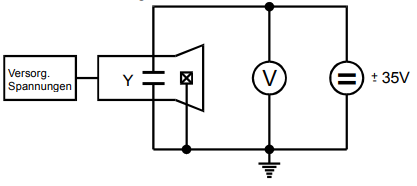
\includegraphics[height=5cm]{schalt1.png}
  \caption{Schaltung zur Untersuchung der Proportionalität zwischen Ablenkspannung und Verschiebung des Auftreffortes. \cite[S.5]{kent}}
\end{figure}

Im zweiten Teil wird ein Kathodenstrahloszillograph nach Abbildung 5 konstruiert. Hierbei wird
die Sägezahnfrequenz so eingestellt, dass auf dem Oszillographen stehende Bilder der angelegten
Sinusspannung zu sehen sind. Die Fälle $n = \frac{1}{2}, 1, 2, 3$ werden realisiert und die
zugehörige Sägezahnfrequenz wird notiert.

\begin{figure}[H]
  \centering
  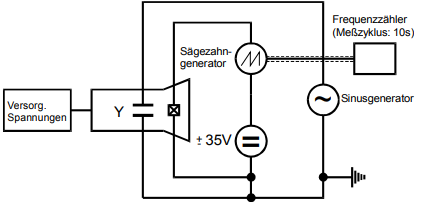
\includegraphics[height=5cm]{schalt2.png}
  \caption{Schaltung zum Bau eines Kathodenstrahloszillographen. \cite[S.5]{kent}}
\end{figure}
